\documentclass[11pt, a4paper]{article}

\usepackage{amsmath}
\usepackage{amssymb}
\usepackage{graphicx}
\usepackage{listings}
\usepackage{color}
\usepackage[section]{placeins}
\usepackage{paralist}
\usepackage{fullpage}

\usepackage{caption}
\usepackage{subcaption}

\definecolor{mygreen}{rgb}{0,0.6,0}
\definecolor{mygray}{rgb}{0.5,0.5,0.5}
\definecolor{mymauve}{rgb}{0.58,0,0.82}

\lstdefinelanguage{JavaScript}{
  keywords={typeof, new, true, false, catch, function, return, null, catch,
switch, var, if, in, while, do, else, case, break},
  keywordstyle=\color{blue}\bfseries,
  ndkeywords={class, export, boolean, throw, implements, import, this},
  ndkeywordstyle=\color{darkgray}\bfseries,
  identifierstyle=\color{black},
  sensitive=false,
  comment=[l]{//},
  morecomment=[s]{/*}{*/},
%  commentstyle=\color{purple}\ttfamily,
%  stringstyle=\color{red}\ttfamily,
  morestring=[b]',
  morestring=[b]"
}

\lstset{ %
  backgroundcolor=\color{white},
  basicstyle=\footnotesize,
  breakatwhitespace=false,
  breaklines=true,
  captionpos=b,
  commentstyle=\color{mygreen},
  escapeinside={\%*}{*)},
  extendedchars=true,
  keepspaces=true,
  keywordstyle=\color{blue},
  rulecolor=\color{black},
  showspaces=false,
  showstringspaces=false,
  showtabs=false,
  stepnumber=2,
  stringstyle=\color{mymauve},
  tabsize=2,
}

\newcommand*{\titleGM}{\begingroup
\hbox{ 
\hspace*{0.2\textwidth} 
\rule{1pt}{\textheight} 
\hspace*{0.05\textwidth} 
\parbox[b]{0.75\textwidth}{ 

{\noindent\Huge\bfseries Mobile Web}\\[2\baselineskip] % Title
{\large \textit{SEM2220 - Assignment 1}}\\[4\baselineskip] % Tagline or further description
{\Large \textsc{Alexander D Brown (adb9)}} % Author name

\vspace{0.5\textheight} 
}}
\endgroup}


\title{Mobile Web}
\author{Alexander D Brown (adb9)}

\begin{document}
\titleGM 
\tableofcontents
\newpage

\section{Introduction}
This report shows the process undertaken to change the Conference Web
Application (produced by Chris Loftus) from a statically generated list to one
loaded dynamically using JavaScript from a Web SQL
database\cite{WebSQL2010Hickson}.

The Conference Web Application is a website which was designed using
progressive enhancement to provide content to mobile devices as well as desktop
browsers. It uses the jQuery Mobile framework\cite{jQueryMobile} to give a 
native feel for mobile users. 

The process involved the implementation of some JavaScript code to query the
Web SQL database created in HTML 5 storage when the Conference Web Application is
initially loaded. The results of this query are then dynamically rendered in
the sessions page as a part of a jQuery Mobile list view.



\section{Implementation}
This section describes the process taken to implement the dynamic loading of
sessions into the session view from the pre-existing Web SQL database. There
were two main steps to do this:

\begin{enumerate}
\item Query the database using standard SQL statements.
\item Render the results of the query.
\end{enumerate}

Because a lot of the code was already written this was a simple case of
implementing two methods. The method to query the database handled the building
of SQL to perform the query and use a callback method to handle the results of
this query. This callback method also needed implemented and read the each of
the results and appended them to a jQuery Mobile list view object using jQuery
methods.

\subsection{Implementing the Database Query}
The \texttt{DataContext.js} file handles the data handling for the application,
on the first load of the whole site the database is built from hard-coded
values in the file. It is also responsible for performing database queries and
transactions and therefore is the location which the sessions query is
required.

To start with a simple SQL statement was designed, based on the hints from the
original author which would select everything from the sessions table where the
session was on the first day of the conference.

\begin{lstlisting}[language=sql]
SELECT * FROM sessions WHERE sessions.day_id = '1'
                       ORDER BY sessions.starttime ASC
\end{lstlisting}

From this it is a simple matter of calling a method from the transaction method
as shown:

\begin{lstlisting}[language=javascript]
var querySessions = function(tx) {
  var sql = // SQL Statement
  tx.execute_sql(sql, [], callback, error_callback);
};
\end{lstlisting}

Where the callback is the rendering function.

To make this statement a little more secure, as recommended by the API, it was
changed to be:

\begin{lstlisting}[language=javascript]
var querySessions = function(tx) {
  var sql = "SELECT * FROM sessions WHERE session.day_id = ? 
             ORDER BY sessions.starttime ASC";
  tx.execute_sql(sql, [1], callback, error_callback);
};
\end{lstlisting}

Though the query is completely isolated from user input, it may not be in the
future.

To enhance this further, joining the days table to include the name of the day
that the session was on. This could have been hard coded in the rendering
function, but again it may not remain limited to the first day so doing this
dynamically will be a benefit in the future.

\begin{lstlisting}[language=javascript]
var querySessions = function(tx) {
  var sql = "SELECT sessions.* days.day FROM sessions, days 
             WHERE sessions.day_id = ? 
             AND days._id = sessions.day_id 
             ORDER BY sessions.dayid 
             AND sessions.starttime ASC";
  tx.execute_sql(sql, [1], callback, error_callback);
};
\end{lstlisting}

The improve the callback functionality, a helper method was used to provide 
only the rows from the results set to the callback as the other two attributes 
are based on non-select SQL statements.

\subsection{Implementing the Rendering Function}
The \texttt{Controller.js} file handles a lot of the application processing,
particularly dynamic jQuery Mobile elements, but also with some geolocation
processing. It is therefore the home of the function to render sessions onto
the correct page.

The rendering function acts as a callback to the aforementioned database query,
and receives a Web SQL \texttt{SQLResultSetRowList} from the query. The 
rendering function then enumerates over each row. From this information a 
series of HTML can be generated and rendered on the page.

First off, using the jQuery API, the element with the correct ID is found on 
the page and bound to a variable. From this raw HTML was appended to this
element, with each individuals attributes inserted at the correct points.
Finally, the bound element is initialised as a jQuery Mobile list view and
refreshed using the API.

To improve this, several helper functions were written; one to convert the
resulting rows from the \texttt{SQLResultSetRowList} to a standard JavaScript
array to allow easier iteration. Such a function would be of use in extending
the application, so it was well worth implementing.

A second function to render an individual session was also implemented, so that
the processing could be abstracted away. This function returned a list item 
HTML element which could then easily be appended to the correct list in the
main function.

\subsection{Problems Encountered}
The main issues found with this assignment related to the Web SQL database. The
specification is very terse and, as such, doesn't contain a lot of information
as to how the methods and objects actually work.

Because of the nature of JavaScript it can be quite difficult to debug, so
working out the problems with the database connection could be quite difficult
on occasion.

The main issue I ran into is there's no formal specification of the SQL
statements Web SQL supports. When writing more advanced queries, particularly
those involving joins between two or more tables, was a matter of constantly
running the query to see if it would work then changing the statement until
some form of correct result was gained.

%\section{Preview}
% TODO Screenshots if there's room

\section{Testing and Debugging}
% TODO Screenshots of the developer view, winre and emulator testing.
The Chrome developer tools were used to debug the conference web application,
an in-browser implementation using Web Inspector.%TODO \cite
There are several similar tools which also use Web Inspector, including wienre,
a locally run webserver which acts very similarly to the developer tools. The
Apple Web Inspector is another similar product.

The Chrome developer tools were the easiest solution as they are native to the
Google family of browsers and provide support without the need for setting up
additional tools.

The Opera mobile browser was used to test the mobile version of the web
application to ensure it viewed correctly on mobile devices. 
The Android emulator was used to test the hybrid application functioned
correctly as a native Android application.

Figure~\ref{fig:dev-tools} shows the use of the Chrome developer tools to debug
the conference web application. These tools have the ability to inspect
different elements to check their styling information, which is useful to check
existing styles are being correctly applied as well as apply new styles on the
fly.

The resources tool provides functionality to visually inspect a Web SQL
database, this is a useful feature to test that all relevant items are
correctly loaded into list views as well as being able to check to state of the
database and the connections to other tables. This was especially useful when
different databases were joined to provide additional information.

The developer tools also include a basic JavaScript console which picks up any
\texttt{console.log} statements inside the code. This made building and
debugging the application a lot easier when the Web SQL database API didn't
provide the needed information to access objects from the database. Instead
these objects could be logged and inspected using this view.

\begin{figure}[p]
\centering
\begin{subfigure}[b]{0.4\textwidth}
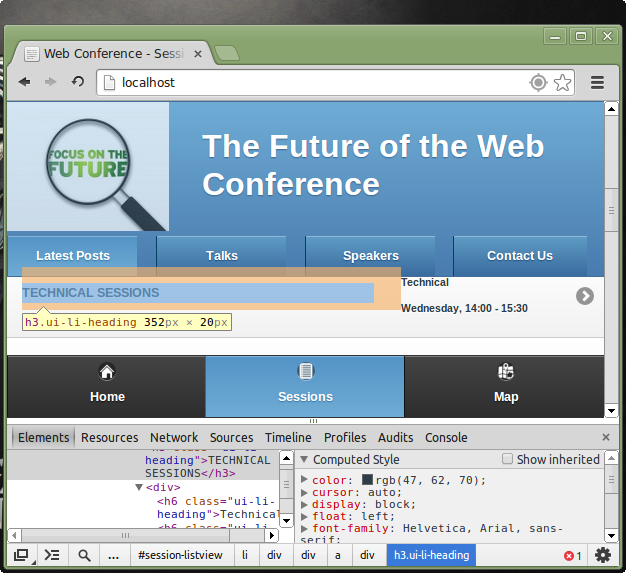
\includegraphics[width=\textwidth]{img/dev-tools-styles}
\caption{Inspecting Element Styles using the Chrome Developer Tools.}
\end{subfigure}
~
\begin{subfigure}[b]{0.4\textwidth}
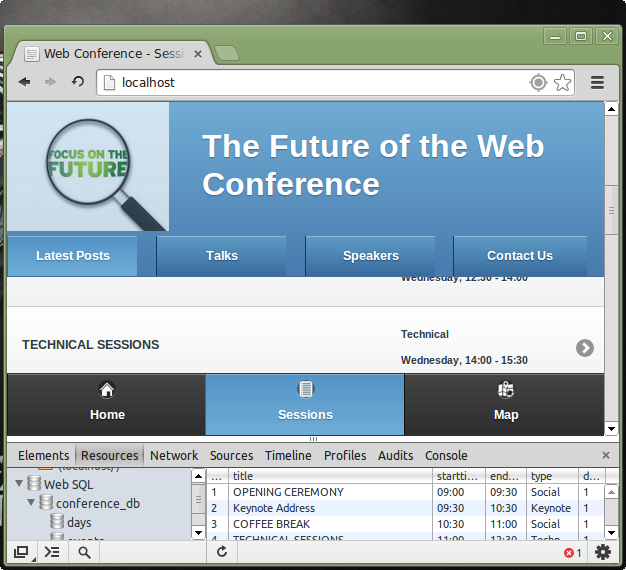
\includegraphics[width=\textwidth]{img/dev-tools}
\caption{Using the Chrome Developer Tools to inspect the database.}
\end{subfigure}
\caption{Using the Chrome Developer Tools for debugging.}
\label{fig:dev-tools}
\end{figure}

Figure~\ref{fig:testing} shows the tools and process used to test the
application in its different formats. The Opera Mobile Emulator provides a
mobile-sized browsers which acts like the Opera Browser package on a mobile
device. This allows the testing of styling and mobile experience as well as
making sure the APIs used are compatible with mobile devices.

The hybrid application was created using PhoneGap and tested on the Android
Emulator. The main bulk of the testing done through this was to ensure the API
worked as part of a native application and not just a web application.

\begin{figure}[p]
\centering
\begin{subfigure}[b]{0.4\textwidth}
\centering
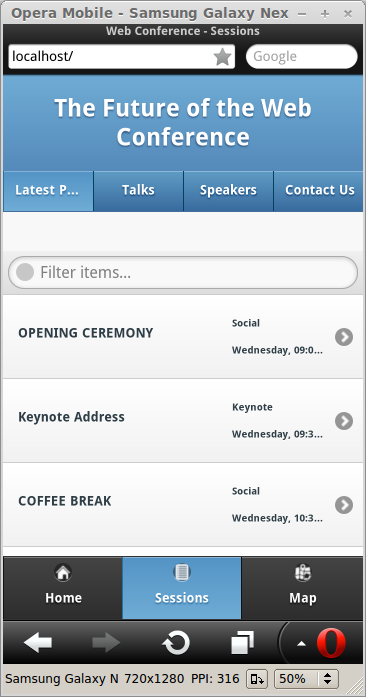
\includegraphics[height=225px]{img/opera-mobile-lists}
\caption{Conference Web Application running as a Website App on the Opera 
         Mobile Emulator}
\end{subfigure}
~
\begin{subfigure}[b]{0.4\textwidth}
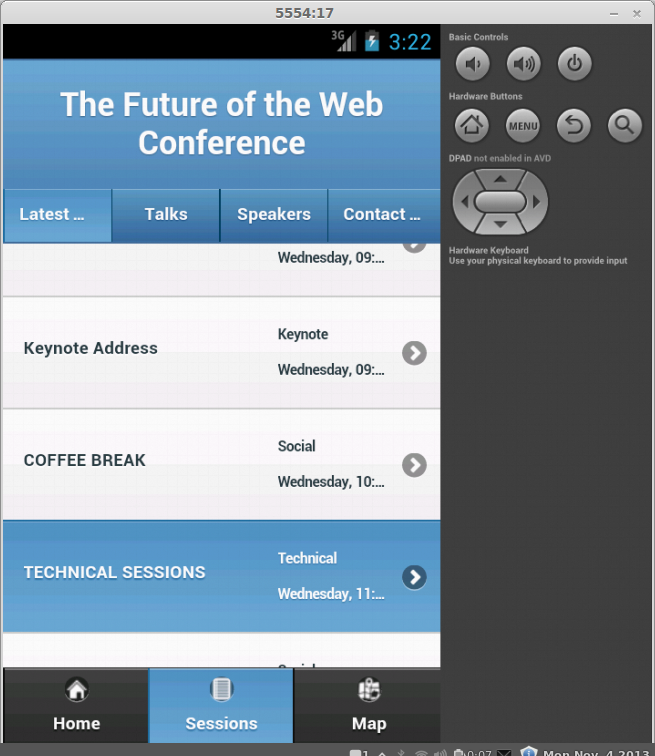
\includegraphics[width=\textwidth]{img/android-lists}
\caption{Conference Web Application running as a Hybrid App on the Android
         Emulator.}
\end{subfigure}
\caption{Testing the Conference Web Application Sessions list on different
         mobile emulators.}
\label{fig:testing}
\end{figure}


\section{Evaluation}
The list view is now dynamically loaded from the Web SQL database and the
quality of the code used is as good as it can be, given the author's
inexperience with JavaScript.

Additional functionality was also added to load the details of a selected
sessions and another level below this to show the talks. Unfortunately this
doesn't appear to work in the Android emulator, possibly due to a bug in the
code or due to a misinterpretation of how jQuery Mobile list view should
function.

Because of this extra functionality the JavaScript is a little messier but has
more helper methods to abstract out too much repeated code. This has hopefully
improved the quality of the code implemented.

The author has learned the basics of jQuery Mobile and Web SQL databases.
jQuery Mobile seems like an interesting set of libraries, but when other, more
recent technologies which are equally, if not better suited, to mobile-first
development (Bootstrap, for example) this knowledge may be of limited use. The
integration with hybrid technologies is a large bonus for the jQuery Mobile
framework.

Web SQL seems like a useful, if somewhat unused technology. It is somewhat
unfortunate that the standard is currently at an impasse as it need an
implementation separate from sqlite. The web storage specification and indexed
database API are cited as two other similar technologies which perform similar
tasks in different ways. Both of these seem like useful libraries and which
could replace the existing implementation of Web SQL in the web application.

Breaking down the mark scheme the author has predicted the grades which should
be gained for each part is shown in table~\ref{tab:marks}

\begin{table}[p]
\centering
\begin{tabular}{| c | c | c |}\hline
\textbf{Part}	& \textbf{Worth}	& \textbf{Predicted Grade} \\ \hline
Documentation	& 30\%			& 25\% \\ 
Implementation	& 50\%			& 45\% \\ 
Flair		& 10\%			& 10\% \\ 
Testing		& 10\%			& 8\% \\ \hline
\textbf{Total}	& 100\%			& 88\% \\ \hline
\end{tabular}
\label{tab:marks}
\end{table}

The author feels a mark of around 88\% should be awarded, the values above were
chosen for the following reasons:

\begin{description}
\item[Implementation] The implementation works to, and beyond, the
specification and is done using the best quality JavaScript the author knows
without a huge amount of experience.
\item[Flair] Additional functionality has been added to the web application.
\item[Testing] Evidence of testing using developer tools and mobile emulators
has been provided in this report.
\item[Documentation] This reports gives the details of the process taken to
implement the dynamic loading of sessions from the Web SQL database and shows
the problems encountered during this process as well as the lessons learned in
the whole project.
\end{description}


\newpage
\bibliographystyle{plain}
\bibliography{citations}

\end{document}
